\section{D-Optimal Designs Without Model Error}\label{section:vanishing}
Our goal in this section is to prove Theorem \ref{thm:char} which
characterizes D-optimal designs when $\modcov = 0$. The necessary
first-order condition for D-optimality of Theorem
\ref{thm:constrained} for $\modcov = 0$ become:

\begin{equation}\label{eq:eigenproblem}
  \sigma^{-2}\fwd \postcov \fwd^* \obs^* = \obs^* \Xi,
\end{equation}
with $\Xi$ diagonal. Equation \eqref{eq:eigenproblem} looks like an
eigenvalue problem for the self-adjoint operator $\sigma^{-2}\fwd
\postcov \fwd^*$, where rows of $\obs$, namely $\meas_j,j=1,\dots, m$,
are eigenvectors. However, $\postcov$ depends on $\obs$ and thus, we
refer to \eqref{eq:eigenproblem} as a \emph{nonlinear} eigenvalue
problem.%%  Proposition \ref{prop:twice woodbury} and Lemma
%% \ref{lemma:sim diag} required 

\begin{proposition}\label{prop:twice woodbury}
  Assume $\fwd \prcov \fwd^*$ is invertible. Then
  \begin{align*}
    \begin{split}
      \fwd( \prcov^{-1} + \sigma^{-2}  \fwd^* \obs^* \obs \fwd )^{-1} \fwd^* 
      %
      %
      = \left ( (\fwd\prcov\fwd^*)^{-1} + \sigma^{-2}  \obs^* \obs \right )^{-1},
    \end{split}
  \end{align*}  
\end{proposition}

\begin{proof}
  The proof amounts to using Woodbury's matrix identity twice and a
  regularization trick. The standard proof for Woodbury's matrix
  identity works for separable Hilbert spaces, as long as all terms
  are well defined. Unfortunately, $\obs^*\obs$ is not invertible, so
  we force it to be. Recall Woodbury's matrix identity:
  \begin{equation}\label{eq:WMI}
    (A + UCV)^{-1} = A^{-1} - A^{-1}U(C^{-1} + VA^{-1}U)^{-1}VA^{-1}. 
  \end{equation}

  Denote:
  \begin{align}\label{eq:notation}
    \begin{split}
      A :&= \prcov^{-1} \\
      U :&= \fwd^* \\
      V :&= \fwd \\
      C :&= \sigma^{-2} (\obs^*\obs+\eps I),\ \eps > 0
    \end{split}
  \end{align}

  Then, by \eqref{eq:WMI}, with the notation \eqref{eq:notation}:
  \begin{equation}\label{eq:first}
  \fwd( \prcov^{-1} + \sigma^{-2}  \fwd^* (\obs^* \obs +\eps I) \fwd )^{-1}\fwd^* = \fwd ( \prcov - \prcov \fwd^* ( \sigma^2(\obs^*\obs + \eps I)^{-1} + \fwd \prcov \fwd^* )^{-1} \fwd \prcov ) \fwd^* \\
      %
      %
      %% &= X - X(\sigma^2Y_{\eps}^{-1} + X)^{-1}X
  %%   \end{split}
  %% \end{align*}
  \end{equation}
  Now, denote:
  \begin{align*}
    X :&= \fwd\prcov \fwd^* \\
    Y_{\eps} :&= \obs^*\obs + \eps I,
  \end{align*}
  and observe that $Y_{\eps}$ is invertible. Substitute $X, Y_{\eps}$
  into the RHS of \eqref{eq:first}:
   \begin{equation}\label{eq:second}
     \fwd( \prcov^{-1} + \sigma^{-2}  \fwd^* (\obs^* \obs +\eps I) \fwd )^{-1}\fwd^* = X - X(\sigma^2Y_{\eps}^{-1} + X)^{-1}X
   \end{equation}

   Note that $X + \sigma^2 Y_{\eps}^{-1}$ is invertible, as the sum of
   two positive definite operators. Now, let
   \begin{align}\label{eq:notation2}
     \begin{split}
       A :&= X^{-1}, \\
       C :&= \sigma^2Y_{\eps}^{-1}, \\
       U :&= I, \\
       V :&= I.
     \end{split}
   \end{align}
   Apply \eqref{eq:WMI} with the notation \eqref{eq:notation2} to the
   RHS of \eqref{eq:second}:
  \begin{align*}
    \begin{split}
      \fwd( \prcov^{-1} + \sigma^{-2}  \fwd^* (\obs^* \obs +\eps I) \fwd )^{-1}\fwd^* &= X - X(\sigma^2Y_{\eps}^{-1} + X)^{-1}X \\
      %
      %
      %
      &= (X^{-1} + \sigma^{-2}Y_{\eps})^{-1} \\
      %
      %
      %
      &= (\fwd \prcov \fwd^* + \sigma^{-2} (\obs^*\obs + \eps I))^{-1}.
    \end{split}
  \end{align*}

  We conclude that $\forall \eps > 0$
  \begin{align*}
    \begin{split}
      \fwd( \prcov^{-1} + \sigma^{-2}  \fwd^* (\obs^* \obs +\eps I) \fwd )^{-1}\fwd^* 
     &= (\fwd \prcov \fwd^* + \sigma^{-2} (\obs^*\obs + \eps I))^{-1}.
    \end{split}
  \end{align*}
  Letting $\eps \to 0$ completes the proof.
\end{proof}


\begin{lemma}[Simultaneous diagonizability]\label{lemma:sim diag}
  Let $\hil$ separable Hilbert space, $C:\hil \to \hil$ self-adjoint
  and $\func_1,\dots,\func_m \in \hil$. Denote $\func^*$ the element
  $\func$ acting as a linear functional. If
  \begin{equation*}
   (C + \sum_{j=1}^m \func_j\func_j^*) \func_l = \xi_l \func_l,\ l = 1,\dots,m
  \end{equation*}
  then $C$ and $\sum_{j=1}^m \func_j \func_j^*$ are simultaneously
  diagonalizable.
\end{lemma}
\begin{proof}
  First, enumerate the eigenvalues of $C + \sum_{j=1}^m
  \func_j\func_j^*$ as $\xi_1,\dots,\xi_\ell$. Denote the indices of
  the eigenvectors corresponding to $\xi_i$
  \begin{equation*}
    S_i := \{ 1 \leq k \leq m | (C + \sum_{j=1}^m \func_j\func_j^* )\func_k = \xi_i \func_k \}.
  \end{equation*}
  Define further
  \begin{equation*}
    A_i := \sum_{k \in S_i} \func_k \func_k^*,
  \end{equation*}
  which is self-adjoint. Two observations are in order. First,
  $\sum_{j=1}^m \func_j\func_j^* = \sum_{i=1}^\ell A_i$. Second, $A_i
  \func_k = 0$ if $k\not \in S_i$, since eigenvectors of different
  eigenvalue are orthogonal. For $k \in S_i$
  \begin{equation}\label{eq:on vi}
    \xi_i \func_k = (C + \sum_{j=1}^m \func_j \func_j^* ) \func_k = (C + A_i) \func_k.
  \end{equation}
  Let $V_i := span \{\func_k \}_{k\in S_i}$. Observe that $V_i$ is
  invariant under $A_i$, by definition, and under $C$, by \eqref{eq:on
    vi}. A second application of \eqref{eq:on vi} shows that $A_i =
  \xi_iI - C$ on $V_i$. This immediately implies $A_i$ and $C$ are
  simultaneously diagonalizable on $V_i$. This holds for every $1 \leq
  i \leq \ell$ and we conclude that $C$ and $A$ are simultaneously
  diagonalizable.
\end{proof}


\begin{proposition}\label{prop:same ev}
  Let $\obs$ satisfy the nonlinear eigenvalue problem
  \eqref{eq:eigenproblem}. Then $\obs^*\obs$ and $\fwd \prcov \fwd^*$
  are simultaneously diagonalizable.
\end{proposition}
\begin{proof}
  \begin{align}\label{eq:mod conditions}
    \begin{split}
      \obs^* \Xi &= \sigma^{-2}\fwd \postcov \fwd^* \obs^*  \text{ (by \eqref{eq:eigenproblem})}\\
      %
      %
      %
      &= \sigma^{-2} \fwd( \prcov^{-1} + \sigma^{-2}  \fwd^* \obs^* \obs \fwd )^{-1} \fwd^* \obs^*  \text{ (by \eqref{eq:postcov})} \\
      %
      %
      %
      &= \sigma^{-2} \left ( (\fwd\prcov\fwd^*)^{-1} + \sigma^{-2}  \obs^* \obs \right )^{-1} \obs^* \text{ (by Proposition \ref{prop:twice woodbury})}.
    \end{split}
  \end{align}

  Now take $\func_j^{*} = \meas_j$ and $C := (\fwd \prcov
  \fwd^*)^{-1}$ and use Lemma \ref{lemma:sim diag}.
\end{proof}

Since we made no assumption regarding the ordering of $\{\lambda_i\}$,
we can denote the corresponding non-zero eigenvalues of $\obs^*\obs$
by $\{\eta_i\}_{i=1}^{k}$ and let $\eta_i = 0$ for $i \geq k+1$.

\begin{proposition}\label{prop:true target}
  Let $\obs$ with $m$ measurements satisfy the nonlinear eigenvalue
  problem \eqref{eq:eigenproblem}. Let $\{\eta_i\}_{i=1}^{\infty}$
  eigenvalues of $\obs^*\obs$ and $\{\lambda_i\}_{i=1}^{\infty}$ the
  corresponding eigenvalues of $\fwd \prcov \fwd^*$. Let $k:=\rank
  \obs^*\obs$. Without loss of generality, let $\eta_i > 0$ for $i\leq
  k$ and $\eta_i = 0$ for $i > k$. Then:
  \begin{enumerate}
    \item $k \leq m$ and $\obs^*\obs$ has exactly $k$ positive
      eigenvalues.
    \item
      \begin{equation*}
        \tar(\obs) = \frac12 \sum_{i=1}^{k} \log (1 + \sigma^{-2}\lambda_i\eta_i) = \frac12 \sum_{i=1}^{m} \log (1 + \sigma^{-2}\lambda_i\eta_i).
      \end{equation*}
    \item Furthermore, if $\obs$ is D-optimal, $\eta_i > 0$ for
      eigenvectors corresponding to the $k$ largest $\lambda_i$.
  \end{enumerate}
\end{proposition}
\begin{proof}
  Part (1) is trivial. To see part (2) holds: 
  \begin{align}
    \begin{split}
      \tar(\obs) &= \frac12\log \det \left (I + \sigma^{-2} \prcov^{1/2} \fwd ^* \obs^*
      \obs \fwd \prcov^{1/2}\right )\\% \text{ (by definition)}\\
      %
      &= \frac12 \log \det \left (I + \sigma^{-2} \obs^* \obs \fwd
      \prcov\fwd^* \right ) \text{ (Sylvester's Determinant
      Theorem)}\\
      %
      %
      %
      &=\frac12 \log \prod_{i=1}^{\infty} ( 1 + \sigma^{-2} \lambda_i\eta_i ) \text{ (Proposition \ref{prop:same ev})} \\
      %
      %
      %
      %&=\frac12 \log \left ( \prod_{i=1}^{k} ( \lambda_i^{-1} + \sigma^{-2} \eta_i )\prod_{i=1}^{k} \lambda_i \right )
      %
      %
      %
      &=\frac12 \sum_{i=1}^{k} \log (1 + \sigma^{-2}\lambda_i\eta_i). 
      %
      %
      %% &=\frac12 \sum_{i=1}^{k} \log(\sigma^2\lambda_i^{-1} + \eta_i) - k\log \sigma + \frac12\sum_{i=1}^k \log \lambda_i.
    \end{split}
  \end{align}
  Part (3) holds since $\log$ is increasing and $\eta_i \geq 0$.
\end{proof}


\begin{proposition}\label{prop:kkt}
  Let $\tar: \mathbb{R}^m \to \mathbb{R}$, $\tar(\eta) =
  \frac{1}{2}\sum_{i=1}^m \log (1+\sigma^{-2}\lambda_i \eta_i)$, with
  $\lambda_i > 0$ and $\sigma^{2} > 0$. Then the maximum of $\tar$
  subject to $\eta_i \geq 0$ and $\sum\eta_i = m$ is obtained at
  \begin{equation}
  \eta_i = \begin{cases}
    \frac{m}{k} - \sigma^2 \lambda_i^{-1} + \sigma^2 \frac{1}{k} \sum_{j\in A} \lambda_j^{-1} & i \in A \\
    0 & i \in A^c
  \end{cases}
  \end{equation}
  where $A:= \{1\leq i \leq m: \eta_i > 0\}$ and $A^c = \{1,\dots, m\}
  \backslash A$, and $k = |A|$, the cardinality of $A$.
\end{proposition}


\begin{proof}
  Let $\Phi(\eta) = \sum_{i=1}^k \eta_i - m$ and $\Omega_j(\eta) =
   -\eta_j$. Then
  \begin{align*}
    \begin{split}
      \frac{\partial \tar}{\partial \eta_i}  &=
       \frac12 \frac{\sigma^{-2}\lambda_i}{1 + \sigma^{-2} \lambda_i\eta_i} = \frac12 \frac{1}{\sigma^{2}\lambda_i^{-1} + \eta_i} \\
      %
      %
      %
      \frac{\partial\Phi}{\partial \eta_i} &= 1 \\
      %
      %
      %
      \frac{\partial \Omega_j}{\partial \eta_i} &= -\delta_{ij}      
    \end{split}
  \end{align*}

  From the KKT conditions, there are $\alpha, \beta_i$ such that for $i=1,\dots,m$:
  \begin{align}
    \begin{split}
      -\frac12 \frac{1}{\sigma^{2}\lambda_i^{-1} + \eta_i} + \alpha - \beta_i  &= 0 \\
      %
      %
      %
      \eta_i &\geq 0\\
      %
      %
      %
      \beta_i &\geq 0\\
      %
      %
      %
      \beta_i \eta_i &= 0\\
      %
      %
      %
      \sum_{i=1}^m \eta_i &= m 
    \end{split}
  \end{align}

  Then, for $i \in A$:
  \begin{align*}
    \begin{split}
      \beta_i &= 0\\
      %
      %
      %
      \sigma^{2}\lambda_i^{-1} + \eta_i  &= \frac{1}{2\alpha}%  \text{ for }  1 \leq i \leq k.\\
      %
      %
      %
      %% \sigma^{-2} \lambda_i &= 2\alpha - 2\beta_i, i \in B \\
    \end{split}
  \end{align*}
  
  Summing over $i \in A$, substituting $\sum_{i\in A} \eta_i =
  \sum_{i=1}^m \eta_i = m$, and dividing by $k:= |A|$:
  $$
  \frac{1}{2\alpha} = \frac{m}{k} + \frac{\sigma^2}{k} \sum_{j\in A} \lambda_j^{-1}.
  %\Rightarrow \alpha = \left ( \frac{2m}{k} + \frac{2\sigma^2}{k}
  %\sum_{i\in A} \lambda_i^{-1} \right )^{-1}.
  $$

  Consequently:
  \begin{align} \label{eq:etas}
    \begin{split}
      \eta_i &= \frac{1}{2\alpha} - \sigma^2 \lambda_i^{-1}\\
      %
      %
      %
      &=\frac{m}{k} + \frac{\sigma^2}{k} \sum_{j\in A} \lambda_j^{-1} - \sigma^2 \lambda_i^{-1}.%\\
      %
      %
      %
      %% &= \frac{m}{k} + \frac{\sigma^2}{k} \sum_{j \in A, j\neq i} \lambda_j^{-1} - \frac{k-1}{k}\sigma^2 \lambda_i^{-1}\\
      %% ,\ i \in A.
    \end{split}
  \end{align}
\end{proof}

The final ingredient we require for the proof of Theorem
\ref{thm:char} is:


\begin{lemma}[Unit norm decomposition]\label{lemma:free}
  Let $M \in \R^{k \times k}$ symmetric positive definite with $\ttr M
  = m$, $m \geq k$. We can find $\func_j \in \R^k,j=1,\dots,m$
  with $\|\func_j\|=1$ and $A = (\func_1,\dots,\func_m)$ such that
  $AA^t = M$.
\end{lemma}

\begin{proof}
  Let us diagonalize $M$, so that $M = U D U^t$ with $D =
  \diag(d_1,\dots,d_k)$ and $U \in \R^{k \times k }$ orthogonal. Let
  $S \in \R^{k \times m}$ with $S_{ii} = \sqrt{d_{i}}$ and zeros
  otherwise. Define $A:= U S V^t$, where $V \in \R^{m \times m}$ is
  orthogonal and will be further restricted later. Then $AA^t = U
  SV^tVS^t U^t = UDU^t$, so $AA^t$ has the required eigenvalues and
  eigenvectors by construction. If we can choose $V$ such that $A$
  also satisfies the unit norm constraints we are done. These
  constraints are, for $j=1,\dots,m$:
  \begin{equation}\label{eq:V constraints}
   1 = [A^tA]_{jj} = [V S^tS V^t]_{jj},
  \end{equation}
  and we can expect to do this since we assumed $\ttr D = m$.

  Define $C = S^tS - I \in \R^{m \times m}$. Note that $\ttr C = 0$ and
  $C$ is diagonal with non-zero entries $d_i-1,i=1,\dots,k$. It suffices
  to find $V$ orthogonal such that $V C V^t$ has zero diagonal. We
  construct such $V$ by sequentially inserting zeros in the diagonal
  and not destroying zeros we already introduced, starting from the
  last diagonal entry and moving to the first. Since $c_{mm} \neq 0$ ,
  let $p < m$ such that $c_{pp}c_{mm} < 0$ (such $p$ exists because
  the trace is zero) and let $\theta \in (0,\pi)$. Define a Givens
  rotation $R^{(m)} \in \R^{m \times m}$ by
  \begin{equation*}
    r^{(m)}_{ab} :=
    \begin{cases}
      1 & a = b \neq p \text{ or } a = b \neq m \\
      \cos \theta & a = b = p  \\
     -\sin \theta & a = p, b = m\\
      \cos \theta & a = b = m \\
      \sin \theta & a = m, b = p \\ 
      0 & o.w
    \end{cases}
  \end{equation*}
  Note that conjugating a matrix by $R^{(m)}$ changes only its $m$ and
  $p$ rows and columns. We want to choose $\theta$ such that
  \begin{equation}\label{eq:mm}
    0 = [R^{(m)} C (R^{(m)})^t]_{mm} = \cos^2 \theta c_{mm} + 2\cos \theta \sin
    \theta c_{mp} + \sin^2\theta c_{pp},
  \end{equation}
  and it suffices to choose $\theta$ such that
  \begin{equation*}
    c_{mm} \cot^2 \theta + 2 c_{mp} \cot \theta + c_{pp} = 0.
  \end{equation*}
  This quadratic in $\cot\theta$ has a real solution, since
  $c_{pp}c_{mm} < 0$ by assumption and we can find $\theta \in
  (0,\pi)$ such that \eqref{eq:mm} is satisfied. We continue to find
  $R^{(m-1)}$ that leaves row and column $m$ unchanged and
  continue introducing zeros to the diagonal. The assumption $\ttr D =
  m \Rightarrow \ttr C = 0$ guarantees we can do that. Taking $V:=
  R^{(1)} R^{(2)} \dots R^{(m-1)}R^{(m)}$ completes the proof.
\end{proof}

\char*

\begin{proof}
  Part (1) is immediate for any measurement operator $\obs$ that
  satisfies the unit norm constraint on measurements. Part (2)
  was proved in Proposition \ref{prop:same ev}. Part (3) was proved in
  Proposition \ref{prop:true target}.
  
  Part (4) is a consequence of Propositions \ref{prop:true target} and
  \ref{prop:kkt}, with the caveat that we did not show that finding
  $\obs$ so that $\obs^*\obs$ has the desired eigenvalues is
  feasible. To this end, we utilize Lemma \ref{lemma:free}: let $M =
  \diag(\eta_1, \dots, \eta_k)$, diagonal with respect to the first $k$
  eigenvectors of $\fwd \prcov \fwd^*$. We take $\obs := A$ from the
  Lemma \ref{lemma:free}.
  
  Recall from \eqref{eq:postcov}, that the posterior precision is
  $\postcov^{-1} = \prcov^{-1} + \sigma^{-2}\fwd^*\obs^*\obs\fwd$. The
  first statement in part (5) now follows from Proposition
  \ref{prop:twice woodbury}, while the second statement follows from
  parts (1) and (4).
\end{proof}


\pgfplotstableread{
  Label     prior  optimal  sub-optimal 
  1         0.2    1.8           1.7
  2         0.8    1.2           0.8
  3         2.2    0             0.5
  4         3.5    0             0.0
}\optimalvsnot

\begin{figure}
  \centering
  \begin{tikzpicture}[scale=0.85]
    \begin{axis}[
        ybar stacked,
        ymin=0,
        ymax=4,
        xtick=data,
        legend style={cells={anchor=east}, legend pos=north west, legend columns=-1},
        reverse legend=false, % set to false to get correct display, but I'd like to have this true
        xticklabels from table={\optimalvsnot}{Label},
        xticklabel style={text width=2cm,align=center},
        legend plot pos=right,
        ylabel={\LARGE precision --- prior and posterior},
        xlabel={\LARGE eigenvector},
      ]
      \addplot [fill=green!80]  table [y=prior,   meta=Label, x expr=\coordindex] {\optimalvsnot};
      \addplot [fill=blue!60]   table [y=optimal, meta=Label, x expr=\coordindex] {\optimalvsnot};     
      \addlegendentry[scale=1.4]{$\sigma^2\lambda_i^{-1}$}
      \addlegendentry[scale=1.4]{optimal $\eta_i$s}
    \end{axis}
  \end{tikzpicture}
  \begin{tikzpicture}[scale=0.85]
    \begin{axis}[
        ybar stacked,
        ymin=0,
        ymax=4,
        xtick=data,
        legend style={cells={anchor=east}, legend pos=north west, legend columns=-1},
        reverse legend=false, % set to false to get correct display, but I'd like to have this true
        xticklabels from table={\optimalvsnot}{Label},
        xticklabel style={text width=2cm,align=center},
        legend plot pos=right,
        ylabel={\LARGE precision --- prior and posterior},
        xlabel={\LARGE eigenvector} ,
      ]   
      \addplot [fill=green!80]  table [y=prior,       meta=Label, x expr=\coordindex] {\optimalvsnot};
      \addplot [fill=blue!60]   table [y=sub-optimal, meta=Label, x expr=\coordindex] {\optimalvsnot};
      \addlegendentry[scale=1.4]{$\sigma^2\lambda_i^{-1}$}
      \addlegendentry[scale=1.4]{sub-optimal $\eta_i$s}
    \end{axis}
  \end{tikzpicture}
  \caption{A comparison of the eigenvalues of the pushforward
    posterior precision $(\fwd\prcov\fwd^*)^{-1} +
    \sigma^{-2}\obs^*\obs$ for a D-optimal design (left) and a
    sub-optimal design (right). Both designs are allowed $m=3$
    measurements. We assume $\sigma^2=1$ and thus, the blue area has
    accumulated height of $\sigma^{-2}m = 3$ in both panels. The
    D-optimal design (left) increases precision where it is
    lowest. The sub-optimal design (right) does not.}
  \label{fig:optimal vs not}
\end{figure}


Theorem \ref{thm:char} facilitates understanding of D-optimal designs
when $\modcov = 0$: Imagine each eigenvector of $\fwd \prcov \fwd^*$
corresponds to a graduated lab cylinder.
%% (Figure \ref{fig:cylinder})
Each cylinder $i$ is filled, a-priori, with green liquid of
$\lambda_i^{-1}$ volume units. We are allowed $m$ measurement, so we
have blue liquid of volume $\sigma^{-2}m$ units at our disposal. When
we seek a D-optimal design, we distribute the blue liquid by
repeatedly adding a drop to whatever cylinder currently has the lowest
level of liquid in it, as long as its index $i \leq m$. The result of
such a procedure is illustrated in Figure \ref{fig:optimal vs not}.
%% \begin{figure}%{r}{0.25\textwidth} 
%%     \centering
%%     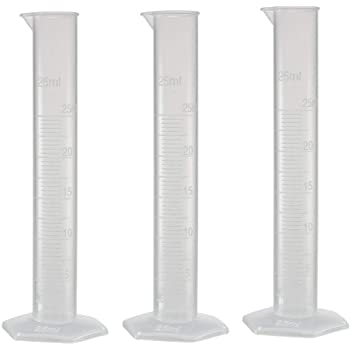
\includegraphics[width=5cm, height=5cm]{cylinders.jpg}
%%     \caption{Three graduated lab cylinders, corresponding to three
%%       eigenvectors. Prior eigenvalues not shown.}
%%     \label{fig:cylinder}
%% \end{figure}


